\documentclass[a4paper]{article}
\usepackage{amsmath}
\usepackage{amssymb}
\usepackage{amsfonts}
\usepackage{graphicx}
\DeclareGraphicsExtensions{.pdf,.eps,.png,.jpg}
\usepackage{color}
\usepackage{psfig}
\usepackage{float}
\usepackage{subfigure}
\setlength\topmargin{0 in}
\setlength\oddsidemargin{0 in}
\setlength\textwidth{6.5 in}

\title{Fully Pipelined AES Core}
\author{Subhasis Das}
\date{}

\begin{document}
\maketitle
\section*{Basic Architecture}
This core meets the NIST FIPS-197 specifications. The basic block diagram is given in Figure \ref{arch}.
\begin{figure}[h]
\centering
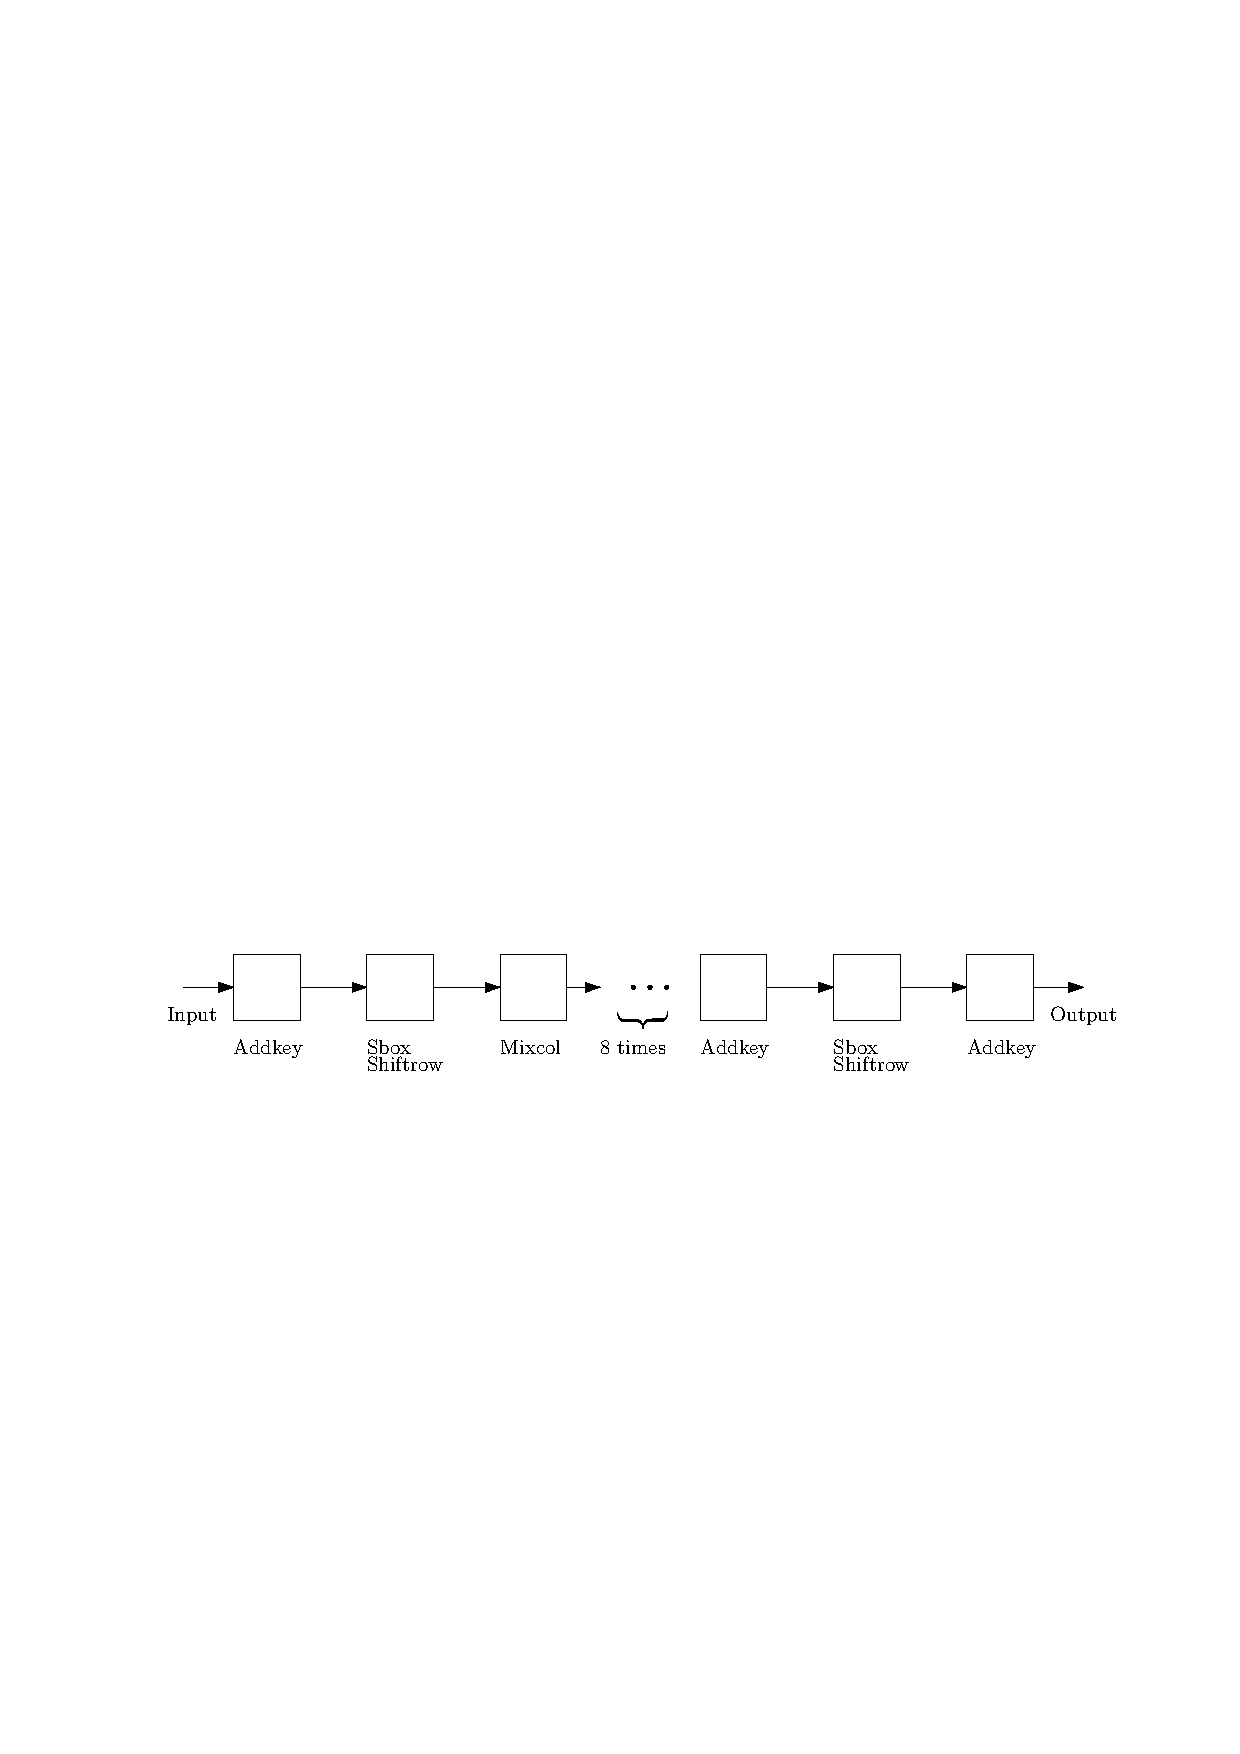
\includegraphics[scale=0.7]{arch}
\caption{Basic Architecture}
\label{arch}
\end{figure}

I have generated each of the roundkeys in two steps. Let us call
\[
\text{RotWord}(\text{ Sbox}(C_3)\;)\text{ xor RCon}\; = \;f(C_3)
\]
Then, we can see that
\begin{equation*}
\begin{aligned}
C_0^\prime &= f(C_3) \;\text{xor}\; C_0 \\
C_1^\prime &= f(C_3) \;\text{xor}\; C_0 \;\text{xor}\; C_1 \\
C_2^\prime &= f(C_3) \;\text{xor}\; C_0 \;\text{xor}\; C_1 \;\text{xor}\; C_2 \\
C_3^\prime &= f(C_3) \;\text{xor}\; C_0 \;\text{xor}\; C_1 \;\text{xor}\; C_2 \;\text{xor}\; C_3
\end{aligned}
\end{equation*}
where $C_i$ is the column i of the current roundkey and $C_i^\prime$ is the column i of the next roundkey.
This first step of generating $f(C_3)$ is done alongwith the addkey step of the previous cycle and the second step is done in the combined S-Box and ShiftRows step.

The inputs to the overall processor are as follows:
\begin{itemize}
\item clk\_i: System Clock, Data I/O at rising edge
\item rst\_i: Asynchronous Reset, active high, initializes all inputs to all stages and the final output to zero.
\item plaintext\_i: 16$\times$8 bits plaintext input
\item keyblock\_i: 16$\times$8 bits keyblock input
\end{itemize}
The output is 
\begin{itemize}
\item ciphertext\_o: 16$\times$8 bits ciphertext output
\end{itemize}

The timing diagram is shown in Figure \ref{clock}.
\begin{figure}[H]
\centering
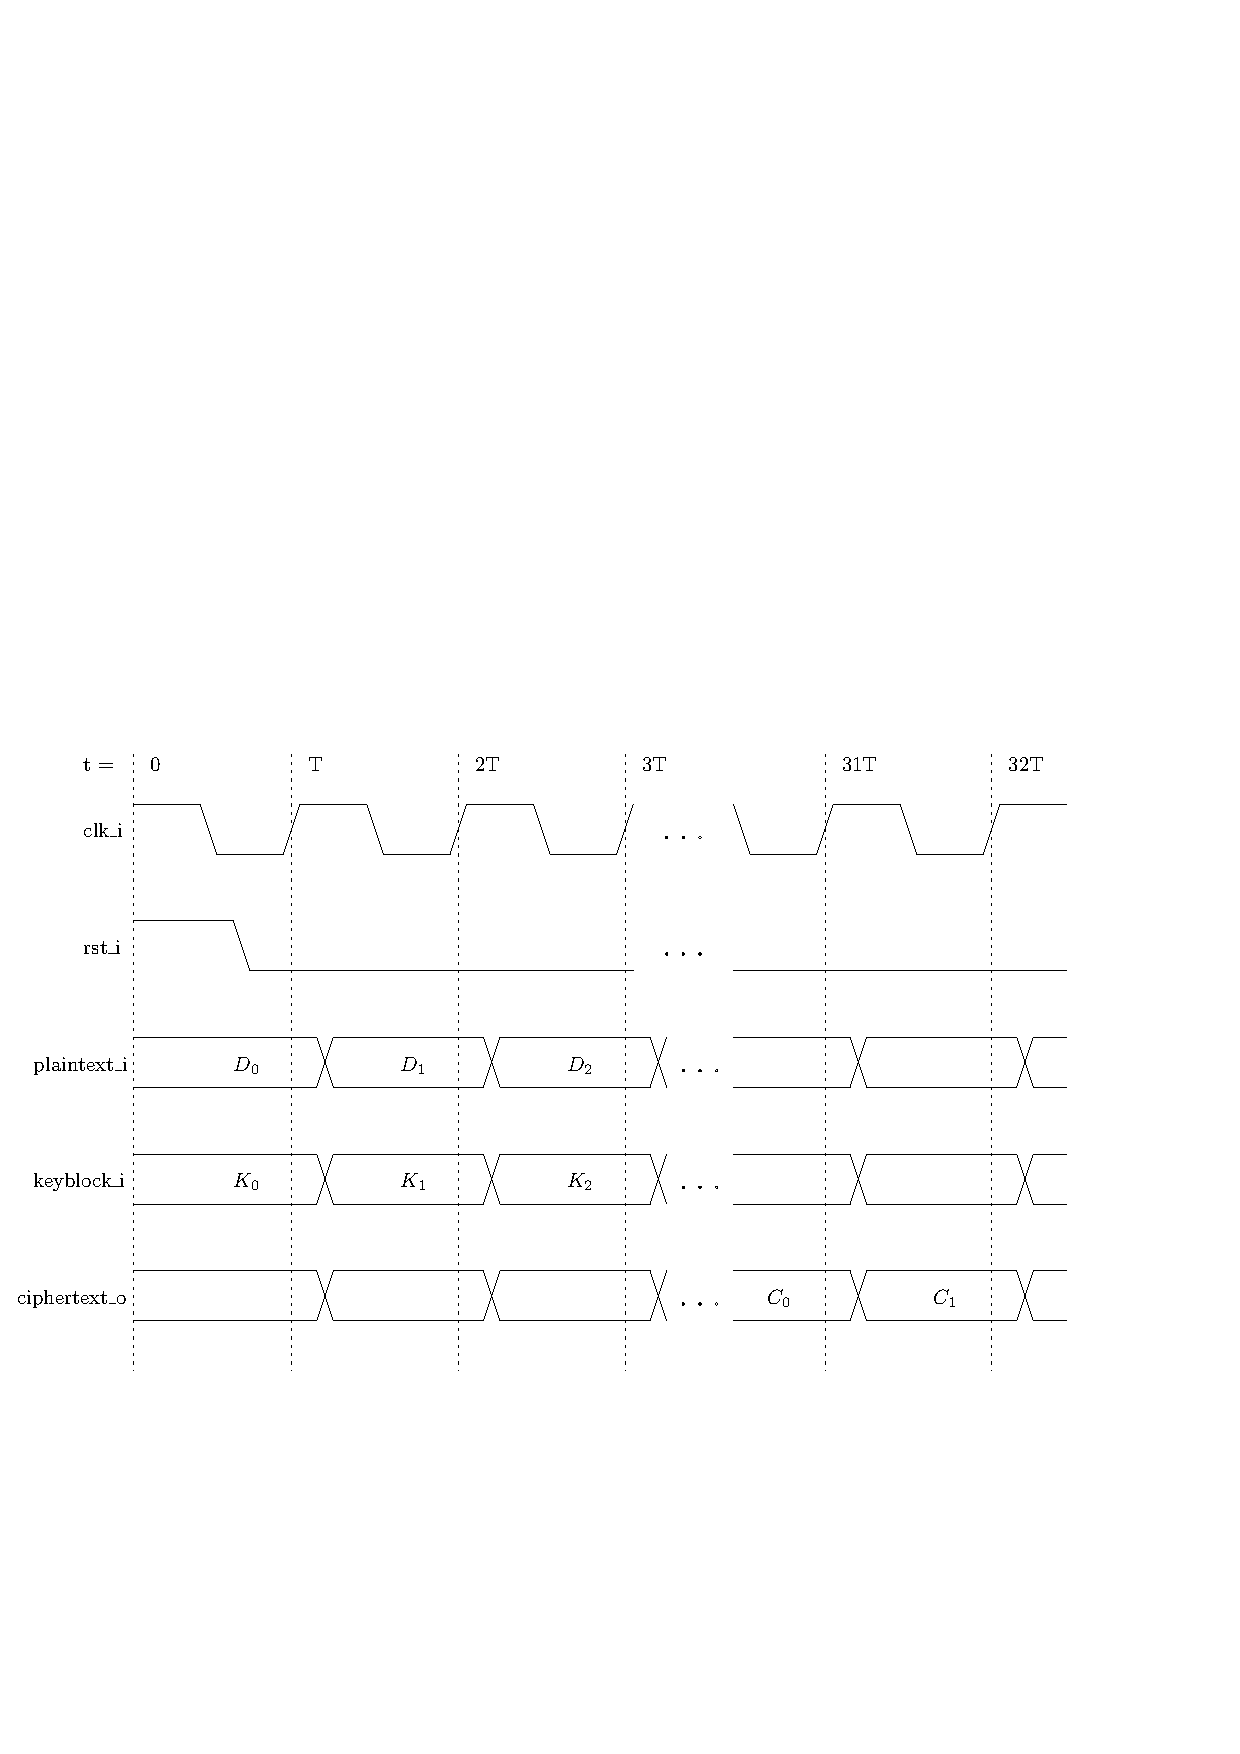
\includegraphics[scale=0.7]{clock}
\caption{Timing Diagram}
\label{clock}
\end{figure}

The \texttt{trunk/rtl/vhdl} directory contains the whole source code.

The sample testbench is in \texttt{trunk/bench/vhdl}.

For compiling and running the testbench, the script \texttt{sim\_isim.sh} in \texttt{trunk/sim/rtl\_sim/run} directory can be used for Xilinx ISim simulator and \texttt{sim\_ghdl.sh} for GHDL. The testbench takes in plaintext and key data from \texttt{vectors.dat} in \texttt{trunk/sim/rtl\_sim/src} directory. The expected ciphertext data should be present in \texttt{cipher.dat} in \texttt{trunk/sim/rtl\_sim/src} directory. The results are written to \texttt{output.log} in \texttt{trunk/sim/rtl\_sim/log} directory. The final line is 'OK' if all tests pass, else it is 'FAIL'. This can be used to automate checkings over large test datasets.

The \texttt{trunk/syn/Xilinx/run} directory contains the \texttt{synth.sh} shell script, which will synthesize the design when run using Xilinx ISE WebPack tools.

The speed optimized synthesis results with timing driven map on a Xilinx 5VLX50T device is shown in Table \ref{stats}.
\begin{table}[h]
\centering
	\begin{tabular}{|l|l|}
	\hline
	$f_{max}$ & $\approx$ 330 MHz  \\
	\hline
	Max throughput & $\approx$ 42 Gbps  \\
	\hline
	Slice Registers's & 7873 (27\%) \\
	\hline
	Slice LUT's & 14724 (51\%) \\
	\hline
	Bonded IOB's & 386 (80\%) \\
	\hline
	\end{tabular}
	\caption{Design Statistics}
	\label{stats}
\end{table}

All the synthesis, map and place and route logs are available in \texttt{trunk/syn/Xilinx/log} directory.
\end{document}
